\chapter{Travail préparatoire et complémentaire à la modélisation de la base de données}

La conception de cette base de données n'a pas pu être possible sans un travail préalable de réflexion et de modélisation, totalement extérieurs à l'utilisation d'\emph{Heurist}. 

\section{Analyse des documents en vue de leur exploitation}

Pour pouvoir tirer un maximum d'informations des factures Rondel, et surtout pour en extraire les données pertinentes à entrer dans la base, il convient d'abord d'analyser la façon dont elles sont structurées. C'est pourquoi a d'abord effectué un travail de consultation et de lecture proche des sources. La lecture attentive, ou \emph{close reading}, est une méthode issue de la critique littéraire consistant en une analyse minutieuse des sources. 
Cependant, le but ici n'est pas de faire une étude exhaustive de la composition des factures, car vu le volume du corpus, ce travail serait trop long à réaliser. Il s'agit simplement, à partir de l'échantillon sélectionné, de repérer quelles sont les informations importantes et récurrentes dans ces factures, afin de réaliser un modèle qui, bien que précis, soit suffisamment général pour pouvoir s'adapter aux différents cas de figure susceptibles d'apparaître dans l'ensemble de ces documents. Plus qu'une obligation, l'absence d'exhaustivité dans l'analyse des documents, puis dans la modélisation des données est même un parti pris, car prendre en compte tous les cas de figure serait impossible, et n'aurait aucun intérêt. Il a donc été établi que les informations qui apparaissent le plus souvent, ainsi que celles permettant d'identifier les factures, les personnes, et surtout les œuvres devront faire partie de la base.

Cette première analyse nous a permis de regrouper certaines catégories d'informations cohérentes entre elles. Cela nous a également fait réfléchir à des premières ébauches de tables de notre future base de données.

Nous nous sommes d'abord concentrés sur les informations qui apparaissent systématiquement concernant les librairies, à savoir leurs noms, adresses et villes. Nous avons également constaté que leur spécialité apparaissait parfois dans les factures, mais que ce n'était pas systématique. 
Nous avons aussi remarqué certaines informations, souvent discrètes, qui concernent des personnes dans les factures. Il s'agit parfois des signataires des documents, ou simplement des personnes mentionnées comme étant propriétaires ou employés de la librairie. Les informations sur les personnes sont particulièrement présentes dans des extraits de correspondances qui se trouvent dans les dossiers à côté des factures. A aussi été envisagée la nécessité de regrouper les informations qui concernent les factures elles-mêmes, telles que leur date, le nombre d'oeuvres achetés dans chaque facture ou les éventuels commentaires parfois inscrits en bas des factures. Dans ce cadre, une attention particulière a été prêtée au montant total, à la date du paiement et à la présence ou non d'un mandat de paiement. Nous avons donc tiré de ces observations la nécessité d'avoir dans notre base une table dédiée aux factures, pour pouvoir retrouver précisément chaque facture, afin de retracer l'origine des informations qui en sont issues. Sont ensuite venues les réflexions sur les données au centre de ce travail sur les factures, à savoir les informations sur les documents achetées par Rondel, qui se trouvent dans les lignes de ces factures. Comme nous l'avons évoqué précédemment, les informations concernant les documents peuvent être multiples (auteur, date, lieu, format, numéro dans le catalogue du libraire) : il a donc fallu les relever de manière exhaustive, pour couvrir tous les cas possibles.

Cette analyse de notre échantillon de factures nous a permis de regrouper les informations les plus importantes, afin de dégager des hypothèses de futures tables de la base de données. Ce travail s'est rapidement suivi de premières modélisations. 

\section{Modélisation et réflexion sur la structure de la base}


Une des étapes nécessaires à la conception d'une base de données est la modélisation, qui consiste à créer la représentation d'un système complexe afin de l'étudier, de le manipuler, de le comprendre. En informatique, modéliser revient donc à établir une logique formelle d'un domaine pour permettre à la machine de le manipuler ou de le calculer\footcite{bermes_2025}.  
Plus que nécessaire, la modélisation est un processus crucial dans la conception d'une base de données, car cela conditionne la structure de la base et influencera donc les performances à venir. Il en existe plusieurs formes, qui correspondent à différents niveaux de précision, et peuvent être réalisées de manière successive lors de la conception d'une base de données. Le premier type, souvent réalisé dans un premier temps, est le modèle conceptuel de données (MCD), qui est une représentation abstraite de la base de données, ayant pour but de modéliser les données qui seront stockées, sans décrire complétement le système. La modélisation conceptuelle se concentre sur les aspects sémantiques du modèle de données, sans aucune indication relative aux structures de stockage ou d'accès aux données\footcite[p. 13]{Soutou_2022}. Le modèle physique présente les données telles qu'elles seront stockées dans la base. Sans négliger le niveau conceptuel, nous avons choisi, dans la modélisation de notre base de données, de nous inspirer de l'étape intermédiaire : le modèle logique de données (MLD), aussi appelé \enquote{schéma relationnel de base de données}\footcite[p. 145]{Bergougnoux_2019}. Plus précis que le modèle conceptuel, ce niveau de modélisation représente les tables de la base de données, et caractérise les liens entre ces tables par la représentation de clés étrangères.



Le modèle de données conçu dans le cadre de notre projet a, dans un premier temps, été réalisé avec le logiciel \emph{Draw.io}\index{draw.io}, outil en ligne de modélisation de diagrammes, particulièrement adapté à la création d'architecture de bases de données, permettant de représenter leur structure\footcite{drawio}. 
Notre modèle est très spécifique : les types de données et les liens entre les tables qu'il décrit ne correspondent pas à ceux que l'on trouve dans des bases de données plus classiques, mais à ceux d'\emph{Heurist}, que nous avons présentés dans le chapitre précédent. Cependant, pour pouvoir représenter de manière précise les liens entre les tables, nous avons choisi de conserver une représentation communément utilisée dans les modèles de données, inspirée du formalisme de Barker, qui est un style graphique de modélisation des données. Les liens entre les tables sont donc représentés par une notation dite \enquote{Crow's foot} (en patte de corbeau), qui permet de modéliser la nature de ces liens par des flèches et des symboles\footcite[p. 7]{Hainaut_2015}. Cette étape peut paraître anecdotique, mais est essentielle car elle va permettre de définir les cardinalités, c'est-à-dire le nombre d'objets concernés par chaque lien\footcite[p. 32]{Soutou_2022}. 
Le modèle de données est visible dans l'annexe A\footnote{Voir \enquote{\nameref{modele donnees}}.}. 


Pour des besoins de clarification, mais également à des fins de communication a été réalisée une représentation simplifiée de ce modèle de données, inspirée des bases \emph{Heurist} précédemment réalisées à la BnF. Ce schéma reprend les différentes tables de la base, et représente par des flèches les liens qui les unissent. Ces flèches se concentrent davantage sur la circulation des données entre les tables que sur la nature des liens. 

\begin{figure}[htbp]
    \centering
    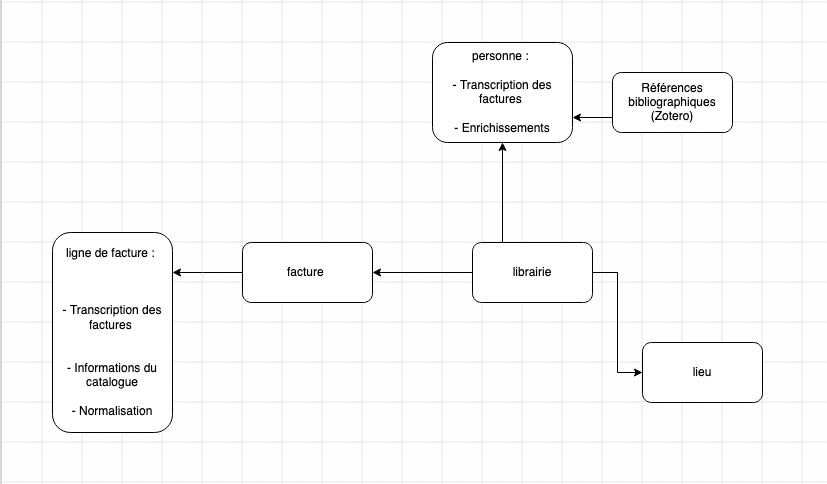
\includegraphics[width=10cm]{Images/modele simplifie.png}
    \caption{Représentation simplifiée du modèle de données.}
    \label{fig:modele-donnees-simplifie}
\end{figure}


Pour ne pas être perdus de vue, les objectifs de la base de données doivent être circonscrits dès le début du projet. Pour ce faire, nous avons utilisé dans ce travail préparatoire un autre outil, moins caractéristique de la modélisation de bases de données, mais plutôt utilisé dans le développement de produits : le \textit{Minimum Viable Product} (MVP). Le principe est de lister les fonctionnalités d'un produit, afin de les hiérarchiser selon un ordre de priorité de développement. Le but principal de cet outil correspondait parfaitement à notre besoin, à savoir d'avoir rapidement un produit fonctionnel pour pouvoir l'expérimenter et recueillir des retours d'utilisateurs\footcite[p. 60]{hervieu_2024}.

Un MVP a donc été réalisé au tout début de ce travail. Les fonctionnalités imaginées ont été partagées en plusieurs catégories. Les \textit{Must have} du projet sont ses éléments essentiels, dont la réalisation a un impact fort et demande un effort acceptable. Les \textit{Can be done} sont réalisables avec un effort minimal et un faible impact sur le projet final. Les fonctionnalités dites \enquote{\textit{Nice to have}} sont supplémentaires et non essentielles. Enfin, les fonctionnalités considérées comme \textit{Out of MVP} sont hors de portée, irréalisables ou constitueraient une grande perte de temps. Ces fonctionnalités ont été représentées par couleur et dans un tableau. Pour des raisons de lisibilité, le document issu de cette réflexion est, lui aussi, disponible dans l' annexe A. Celui-ci a été schématisé sur \emph{draw.io}\index{draw.io}, dans un tableau assorti d'une légende\footnote{Voir \enquote{\nameref{MVP}}}. 


Pour résumer cette réflexion, il a surtout été établi que la priorité absolue, dans la conception de cette base de données, était de reprendre toutes les données venant des factures. Les autres fonctionnalités imaginées n'étaient pas obligatoires, et pouvaient être réalisées dans l'immédiat si le travail n'était pas trop long à faire, ou plus tard. 

\section{Réception et utilisations de cette base de données}

Que ce soit en amont de sa création, tout au long de la modélisation ou de la conception de cette base de données, il convient de prendre en compte les besoins de ses potentiels utilisateurs. Le besoin d'un travail facilitant la recherche et l'exploitation de données sur les factures Rondel est, nous l'avons vu, clairement exprimé au sein du département des Arts du spectacle. 
Cependant, il est parfois nécessaire de centrer notre réflexion sur les usages individuels de la base, à l'échelle de l'utilisateur. 
Nous nous sommes donc inspirés des \textit{Personae}, méthode notamment utilisée dans la conception d'applications informatiques telles que des bibliothèques numériques, consistant à créer des archétypes d'utilisateurs probables d'un produit\footcite{Brangier_2012}. Même si les utilisateurs factices que nous avons imaginés n'ont pas vocation à être exhaustifs, cet outil nous aide à anticiper quelques besoins éventuels auxquels pourrait répondre la base. Le premier utilisateur potentiel est chargé de collection au département des Arts du spectacle, et a une très bonne connaissance de la collection Rondel. Cependant, il n'a pas de formation en informatique, et a besoin d'un outil simple d'utilisation et sans code. Nous avons aussi pensé à un utilisateur qui mènerait un travail de recherche sur la collection Rondel, et qui aurait besoin de cette base pour avoir des informations précises sur le sujet. Cette base pourrait également servir à un potentiel descendant d'une famille de libraires chez qui Rondel se fournissait, et qui souhaite plutôt utiliser cette base comme un outil généalogique. Enfin, cette base pourrait être utile à tout chercheur spécialiste du théâtre, de l'histoire du livre, de l'édition ou de la librairie, qui s'intéresse à la circulation du livre et à des exemplaires en particulier, ou encore à l'histoire économique du livre. 

Afin d'évaluer sa pertinence \emph{a posteriori}, des tests ont aussi été réalisés sur la base de données une fois aboutie. Hélène Keller a saisi dans la base plusieurs factures extérieures à l'échantillon de départ, afin de vérifier si le modèle pouvait s'appliquer à tout le corpus. Malgré tout, ces tests ne permettent pas de certifier que la base de données pourrait couvrir tous les cas possibles, le corpus étant trop volumineux pour cela. 


Ainsi, les différentes étapes de ce travail préparatoire à la modélisation de la base de données ont consisté à analyser les documents, à en extraire les informations les plus importantes et réccurentes, puis à les organiser, ce qui suppose aussi un travail de sélection. S'il est nécessaire d'accorder une place centrale aux sources, il convient également de prendre en compte les besoins des utilisateurs, et d'y rester attentif tout au long du travail. 
